\documentclass[border=1pt]{standalone}
\usepackage{amsmath,amssymb}
\usepackage{tikz}
\usetikzlibrary{arrows.meta,decorations.markings,calc}
\definecolor{cplus}{RGB}{0,114,178}    % blue   (event horizon)
\definecolor{cminus}{RGB}{213,94,0}    % vermilion (inner horizon)
\definecolor{cinf}{RGB}{80,80,80}      % grey   (large loop)
\tikzset{
  mid/.style={decoration={markings,mark=at position #1 with {\arrow{Stealth[length=4.5pt,width=4pt]}}},postaction={decorate}},
  mid/.default=0.5,
  dot/.style={circle,fill,inner sep=1.2pt},
  odot/.style={circle,draw,fill=white,inner sep=1.2pt},
}
\begin{document}
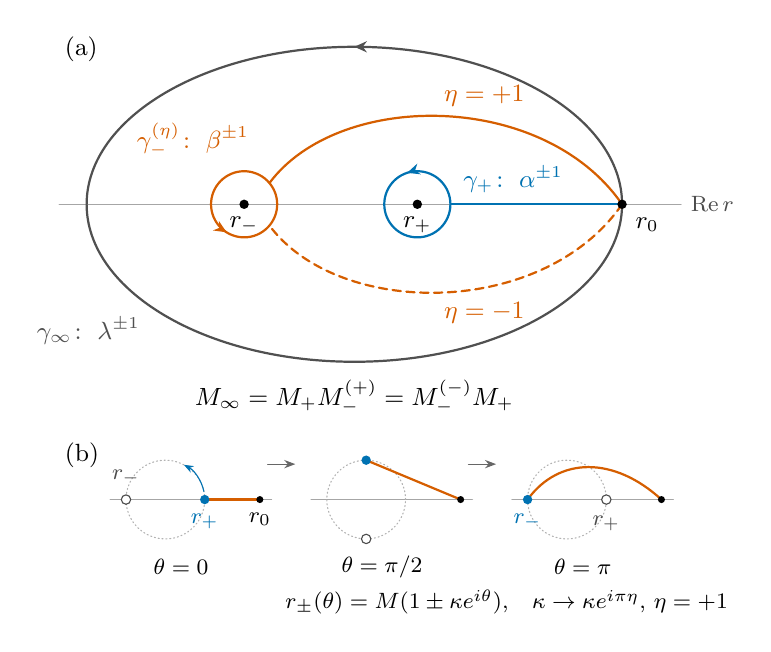
\begin{tikzpicture}[font=\small,line cap=round]
%=============================== (a) monodromies ===============================
\coordinate (rm) at (2.2,0); \coordinate (rp) at (4.4,0); \coordinate (r0) at (7.0,0);
\draw[black!35,thin] (-0.15,0) -- (7.75,0) node[right,black!70,font=\footnotesize] {$\mathrm{Re}\,r$};
% large loop gamma_infinity (counterclockwise, through r0)
\draw[cinf,thick,mid=0.25] (r0) arc[start angle=0,end angle=360,x radius=3.4,y radius=2.0];
\node[cinf,anchor=north east] at (1.0,-1.32) {$\gamma_\infty\!:\ \lambda^{\pm1}$};
% gamma_+ : lasso around r_+ (tail along the axis)
\draw[cplus,thick] (r0) -- ($(rp)+(0.42,0)$);
\draw[cplus,thick,mid=0.3] ($(rp)+(0.42,0)$) arc[start angle=0,end angle=360,radius=0.42];
\node[cplus,anchor=south west] at (4.86,0.02) {$\gamma_+\!:\ \alpha^{\pm1}$};
% gamma_-^{(+)} : tail above r_+   (eta = +1)
\draw[cminus,thick] (r0) .. controls (6.0,1.45) and (3.4,1.45) .. ($(rm)+(40:0.42)$);
% gamma_-^{(-)} : tail below r_+   (eta = -1)
\draw[cminus,thick,dash pattern=on 3pt off 2pt] (r0) .. controls (6.0,-1.45) and (3.4,-1.45) .. ($(rm)+(-40:0.42)$);
% loop around r_-
\draw[cminus,thick,mid=0.55] ($(rm)+(40:0.42)$) arc[start angle=40,end angle=400,radius=0.42];
\node[cminus,anchor=south] at (1.55,0.48) {$\gamma_-^{(\eta)}\!:\ \beta^{\pm1}$};
\node[cminus,anchor=south] at (5.25,1.12) {$\eta=+1$};
\node[cminus,anchor=north] at (5.25,-1.12) {$\eta=-1$};
% points
\node[dot,label={[font=\small,label distance=-1pt]below:$r_-$}] at (rm) {};
\node[dot,label={[font=\small,label distance=-1pt]below:$r_+$}] at (rp) {};
\node[dot,label={[font=\small]below right:$r_0$}] at (r0) {};
\node[anchor=north west,font=\small] at (-0.2,2.25) {(a)};
% relation
\node[font=\small] at (3.6,-2.45) {$M_\infty=M_+M_-^{(+)}=M_-^{(-)}M_+$};
%=============================== (b) exchange ===============================
\begin{scope}[yshift=-3.75cm]
\node[anchor=north west,font=\small] at (-0.2,0.85) {(b)};
\foreach \k/\th/\lab in {0/0/{$\theta=0$}, 1/90/{$\theta=\pi/2$}, 2/180/{$\theta=\pi$}}{
  \begin{scope}[xshift=0.35cm+\k*2.55cm]
    \coordinate (c) at (0.85,0);
    \coordinate (A) at ($(c)+(\th:0.5)$);     % moving event horizon r_+(theta)
    \coordinate (B) at ($(c)+(\th+180:0.5)$); % moving inner horizon r_-(theta)
    \coordinate (z) at (2.05,0);
    \draw[black!35,thin] (0.15,0) -- (2.2,0);
    \draw[black!30,densely dotted] (c) circle[radius=0.5];
    \ifnum\k=2
      \draw[cminus,thick] (A) .. controls (0.75,0.55) and (1.45,0.55) .. (z);
    \else
      \draw[cminus,thick] (A) -- (z);
    \fi
    \ifnum\k=0
      \draw[cplus,-{Stealth[length=3.5pt]}] ($(c)+(12:0.5)$) arc[start angle=12,end angle=62,radius=0.5];
    \fi
    \node[dot,cplus] at (A) {};
    \node[odot,draw=black!70] at (B) {};
    \node[dot,inner sep=0.9pt] at (z) {};
    \node[font=\footnotesize] at (1.05,-0.85) {\lab};
  \end{scope}
}
% labels on the first and last frames
\node[cplus,font=\footnotesize,anchor=north] at (0.35+1.35,-0.06) {$r_+$};
\node[font=\footnotesize,anchor=south,black!70] at (0.35+0.35,0.06) {$r_-$};
\node[font=\footnotesize,anchor=north] at (0.35+2.05,-0.04) {$r_0$};
\node[cplus,font=\footnotesize,anchor=north] at (0.35+5.1+0.35,-0.06) {$r_-$};
\node[font=\footnotesize,anchor=north,black!70] at (0.35+5.1+1.35,-0.08) {$r_+$};
% arrows between frames
\draw[-{Stealth[length=4pt]},black!60] (2.5,0.45) -- (2.85,0.45);
\draw[-{Stealth[length=4pt]},black!60] (5.05,0.45) -- (5.4,0.45);
\node[font=\footnotesize,anchor=west] at (2.6,-1.3) {$r_\pm(\theta)=M(1\pm\kappa e^{i\theta})$,\quad $\kappa\to\kappa e^{i\pi\eta}$, $\eta=+1$};
\end{scope}
\end{tikzpicture}
\end{document}
